%
% PKUMpLtX --- A LaTeX document class for 'Modern Physics Laboratory' in PKU based on `revtex4-2`
%
% Please read `README.md' and the template file before using
% 需要确保 font 选项指定的字体已安装! 具体参见 `README.md' 的说明.
\documentclass[font=default]{mpltx}

% 以下至 \begin{document} 都仅是本文件为了方便额外定义的命令, 写报告时不需要.
\hypersetup{colorlinks=true}% 超链接带颜色
\usepackage{xcolor}
\newcommand{\note}[1]{{\color{gray}#1}}
\NewDocumentCommand{\pkg}{s o m}{%
    \IfBooleanF{#1}{%
        \IfNoValueTF{#2}%
            {\href{https://www.ctan.org/pkg/#3}}%
            {\href{https://www.ctan.org/pkg/#2}}%
    }%
    {\textsf{#3}}%
}
\newcommand*\cs[1]{\texttt{\textbackslash #1}}
\newcommand*\env[1]{\textit{\texttt{#1}}}
\newcommand*\code[1]{\texttt{#1}}
\newcommand*\file[1]{\textbf{\texttt{#1}}}
\makeatletter
\newcommand\releasedate{%
    \href{https://github.com/CastleStar14654/PKUMpLtX/releases/tag/\mpltx@fileversion}%
        {\mpltx@filedate, \mpltx@fileversion}}
\makeatother
% 以上是本文件为了方便额外定义的命令, 写报告时不需要.

\begin{document}

\title{约瑟夫森效应实验} % 切合报告内容, 简短明确, 可以不同于讲义
\author{郑熔} % 这里 \emailphone 一定要紧跟在 \author 后方
\emailphone{2300011359@stu.pku.edu.cn}{(86)19805861588}
% 如果改用 \email 则仅需要邮箱参数
\affiliation{北京大学物理学院\quad 学号: 2300011359}
% % 可以使用 \zhdate 自动生成中文日期, 如
\date{\zhdate{2025/9/10}}
% % 也可使用 babel 的 \localedate, 如
% \date{\localedate{2020}{12}{1}}
% % 两者均会输出 `2020 年 12 月 1 日'
% 下面的 \date 的参数是为了自动输出正确版本号, 正式报告请替换为上面的两种 \date 之一
% \date{\releasedate}
\begin{abstract}
  超导现象是指当温度下降到某一临界温度以下时, 材料展现出零电阻特性和完全抗磁性, 这是超导态的两个基本特性.
  超导电性源于电子的配对和相干凝聚, 常规低温导体两电子之间通过声子作用相互吸引, 形成库珀对.
  约瑟夫森效应是指两块超导体被一绝缘薄层分开时库珀对的量子隧穿现象, 分为直流约瑟夫森效应和交流约瑟夫森效应, 在量子电压基准, 超导量子电路, 高灵敏度测量仪器等领域有重要应用.
  本实验测量高温超导体$YBa_2Cu_3O_{7-x}$超导临界电流, 观测直流约瑟夫森效应得到77K温度下的约瑟夫森临界电流, 以及观察微波辐照下的交流约瑟夫森效应并测量得到微波频率, 验证了约瑟夫森效应理论的正确性.

  % \note{本文档为对 \href{https://github.com/CastleStar14654/PKUMpLtX}{\pkg*{PKUMpLtX}} 的使用示例, 灰色部分为额外针对 \LaTeX{} 模板使用的说明或是一些能提升输出效果的琐碎细节.
    % 也请注意查看源文档 \file{template.tex} 中的注释.}
\end{abstract}
\keywords{约瑟夫森效应, 超导, 双晶约瑟夫森结}

\maketitle

\section{引言}

  1911年荷兰物理学家昂内斯 (H. Kamerlingh Onnes) 在研究汞的电阻率时发现, 当温度降低到4.2K时, 汞的电阻率突然降为零, 这种现象被称为超导现象.
  零电阻特性和完全抗磁性是超导态的两个基本特性, 分别是指超导体在超导态下电阻为零, 超导体在超导态下能完全排斥外加磁场.
  超导体根据其临界温度与液氮温度的关系可以分为低温超导体和高温超导体. 
  1957年美国三位科学家巴丁 (J.Bardeen) 、库珀 (L.N.Cooper) 和施里弗 (J.R.Schrieffer) 提出了BCS理论, 揭示了超导电性源于库珀对 (Cooper pair) 的相干凝聚.
  其中, 常规低温导体两电子之间通过声子作用相互吸引, 形成库珀对; 而对于非常规的高温超导体, 其库珀对的形成机制尚未完全弄清.
  1962年, 约瑟夫森 (B. D. Josephson) 预言了两块超导体被一绝缘薄层分开时库珀对的量子隧穿现象, 即约瑟夫森效应, 分为直流约瑟夫森效应和交流约瑟夫森效应.
  直流约瑟夫森效应是指在没有加电压的情况下, 超导电流可以通过绝缘层隧穿, 其最大值称为约瑟夫森临界电流, 交流约瑟夫森效应是指当在约瑟夫森两端电压不为 0 时, 仍然有通过结的超导隧穿电流, 频率为$f=2eV/h$, 其中$e$为元电荷, $h$为普朗克常数.
  约瑟夫森效应是宏观量子效应的重要体现, 在量子电压基准, 超导量子电路, 高灵敏度测量仪器等领域有重要应用\cite{jindaiwulishiyan}.
  \par 本实验使用的约瑟夫森结为高温超导体$YBa_2Cu_3O_{7-x}$材料以双晶衬底方式实现弱连接构成的双晶约瑟夫森结. 实验首先测量了该双晶约瑟夫森结的超导临界温度; 接着观察直流约瑟夫森效应, 得到约瑟夫森临界电流; 最后给约瑟夫森结加微波辐照而观察到夏皮罗台阶, 即交流约瑟夫森效应, 并测量得到微波频率.
  通过对以上现象的观察, 可以进一步加深对超导现象、约瑟夫森效应以及宏观量子现象的理解.
  \begin{figure}[htbp]
    \centering
    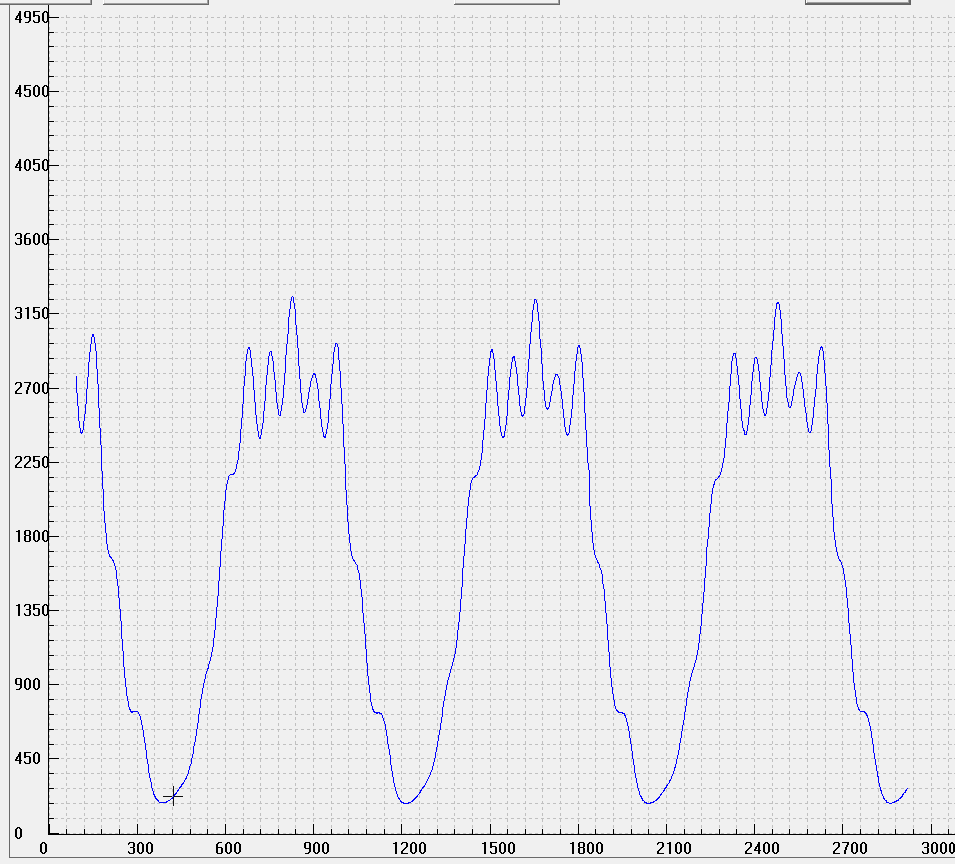
\includegraphics[width=0.85\linewidth]{fig/2.png}
    \caption{双晶约瑟夫森结示意图:(a)双晶衬底,其晶界两侧品粒的品轴(平行于衬底表面)取向不同,夹角为$\delta$.(b)在双晶衬底上外延生长超导薄膜,然后在晶界附近刻蚀出超导微桥形成双品约瑟夫森结.(c)双晶约瑟夫森结的俯视示意图,其中包括和双晶结相连的测试电极以实现标准的四引线法测量.
      % \note{推荐使用相对大小插入图片, 比如这里是 0.8 倍当前区域文字宽度 (\cs{linewidth}).
      %   推荐对实验装置图和数据图使用矢量图插入}
      }

    \label{fig:shuangjinjie}
  \end{figure}


% 研究论文引言一般包含以下内容:
% 所研究领域背景和现状,
% 有待研究的问题,
% 本研究的物理目的和主要方法.
% 通过空行或者 \par 命令分段. 本行不是空行, 没有分段效果
% 引言一定要切合报告正文, 不能漫无目的地介绍背景, 要快速地将读者引导到报告主题上.
% 引言篇幅可以在较大范围内变化, 但最长不应超过报告文字篇幅的1/3.

% 引言撰写可以参考实验讲义和资料, 可以概括复述, 但不能抄.
% \note{这里是一个对实验教材 \cite{jindaishiyan} 的引用示例.}
% \note{注意在 \cs{cite} 命令前后适当添加空格.
%   可以连续引用.
%   引用标记要出现在标点之前 \cite{GBT7714,pr}.
%   引用处理使用 \textsc{Bib\TeX};
%   对于外文期刊, \file{*.bib} 格式的引用数据很容易从出版商获得;
%   \href{https://scholar.google.com}{Google 学术}和\href{https://xueshu.baidu.com}{百度学术}等文献搜索引擎也提供以\file{*.bib} 格式导出的功能.
%   这里是对首次探测到引力波的报道的引用 \cite{PhysRevLett.116.061102}.}

% \section{理论}\label{sec:theory}

% 可选, 概括本实验必须的理论.
% 也可以适当地给出必要的公式, 公式应编号.
% \note{自然对数的底、虚数单位以及圆周率国标 \cite{GBT3102.11} 和 ISO \cite{ISO80000-2} 都推荐为正体 (虽然国际学界并不怎么实行这点), 本模板提供了 \cs{ii}, \cs{ee}, \cs{jj}, \cs{uppi} 作为简写, 如
%   \begin{equation}\label{eq:1}
%     \ee^{\ii\uppi}+1=0.
%   \end{equation}
%   注意公式应作为句子的一部分在末尾给出必要的标点符号.
%   上式可以交叉引用为\autoref{eq:1}.}

% \note{此外, 摄氏度和度在2020年初后已可在 \LaTeX{} 中的非数学模式直接打出 \cite{fntguide},
%   比如 \cs{textdegree} (\textdegree) 和 \cs{textcelsius} (\textcelsius, 虽然国际计量局 \cite{si} 和 Unicode 联盟 \cite{unicode} 都更推荐使用 \code{\textbackslash{}textdegree\{\}C} 的写法, 写成 \textdegree{}C).
%   再比如, \cs{textmu} (\textmu) 可以给出微米需要的正体词头符号.
%   你也可以使用 \pkg{siunitx} 宏包 (参见 \file{README.md}) 来帮助你管理单位格式.}

\section{实验装置}
\subsection{实验装置示意}

  实验装置主要分为三个部分, 测量系统 (约瑟夫森效应观测仪, DH1121C型微波信号源, 惠普33120A函数发生器) , 记录系统 (TYPE3086X-Y RECORDER) 和降温系统 (液氮罐, 样品杆) .其中约瑟夫森效应观测仪主要包括恒流源、定值电阻及相应的测试线路和控制开关. 样品杆上内部装有铂电阻温度计和待测样品. 

% 在此部分需要成段介绍实验方法和条件 (不是罗列操作步骤), 交待清楚到别人能重复你的实验结果的程度.
% 此外, 还需表明你已尽了最大努力来提高实验精度和结果的可靠性 (简单的不确定度估计可以在此节给出, 复杂一些的可以放到分析讨论部分).

% 首先应给出一个实验装置示意图.
% 例如, 如下同学的示意图\autoref{fig:instruments} 非常清晰, 值得借鉴 (各关键部件也可标在图中).

\begin{figure}[htbp]
  \centering
  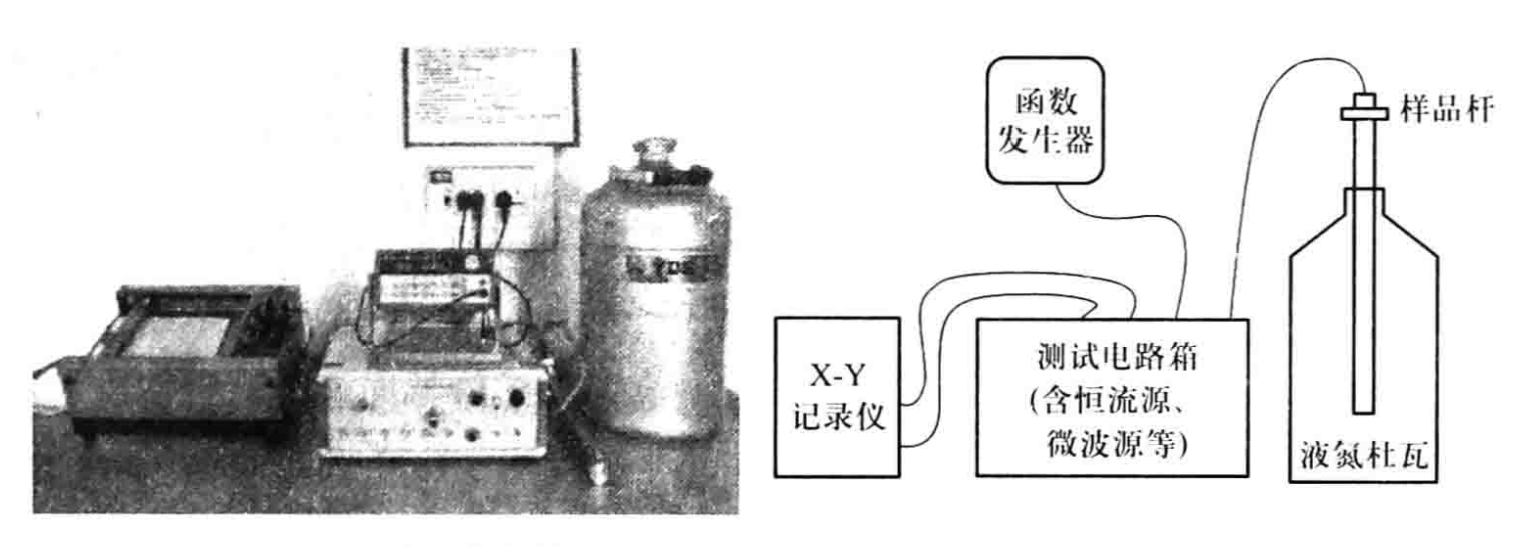
\includegraphics[width=0.85\linewidth]{fig/1.png}
  \caption{约瑟夫森效应测试装置实物图 (左) 和结构示意图 (右).
    % \note{推荐使用相对大小插入图片, 比如这里是 0.8 倍当前区域文字宽度 (\cs{linewidth}).
    %   推荐对实验装置图和数据图使用矢量图插入}
    }
  \label{fig:dianlu}
\end{figure}

  其中, 测量系统和记录系统之间的连接示意图如\autoref{fig:dianlu} 所示.
  \par
  当测量约瑟夫森结的$R-T$曲线时, $X-Y$记录仪的x轴输入为铂电阻温度计两端电压$V_T$, y轴输入为约瑟夫森结两端电压$V_J$. 给铂电阻温度计供电的恒流源输出电流为$0.9mA$, 
  给约瑟夫森结供电的恒流源输出电流为$50\mu A$. 由铂电阻两端的电压和通过铂电阻的电流可以计算出铂电阻的电阻值$R_T=V_T/I_T$, 再查铂电阻电阻值和温度的关系表可以得到每个时刻的温度.
  由约瑟夫森结两端的电压和通过约瑟夫森结的电流可以计算出约瑟夫森结的电阻值$R_J=V_J/I_J$. 由此可以得到约瑟夫森结的$R-T$曲线.
  \par
  当测量约瑟夫森结的$V-I$曲线时, $X-Y$记录仪的x轴输入为定值电阻两端电压, y轴输入为约瑟夫森结两端电压$V_J$. 
  根据定值电阻两端电压和定值电阻的阻值可以得到流过约瑟夫森结的电流, 由此可以画出约瑟夫森节两端电压和流过它的电流的关系图$V-I$曲线.
  
  \begin{figure}[htbp]
  \centering
  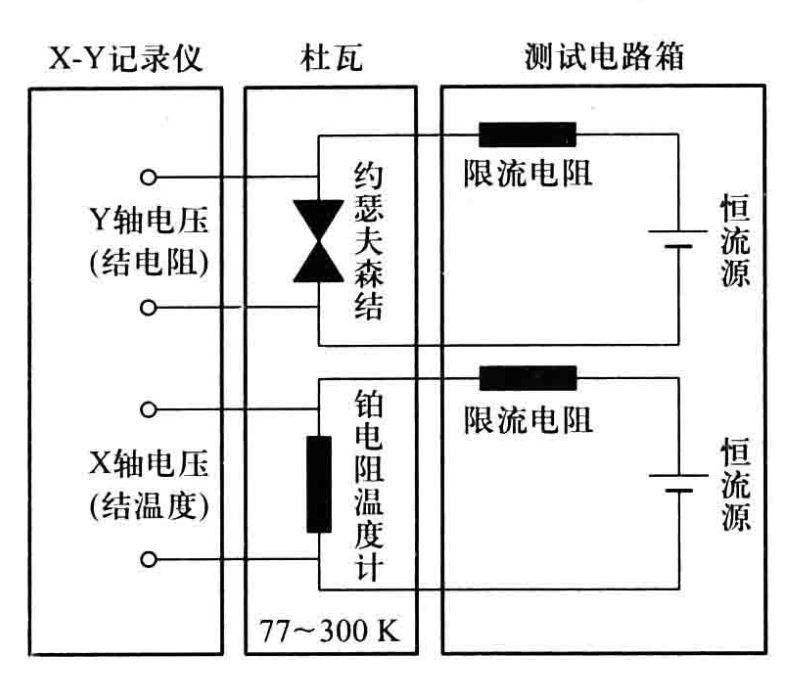
\includegraphics[width=0.85\linewidth]{fig/RTconnect.png}
  \caption{$R-T$曲线测量原理示意图
    % \note{推荐使用相对大小插入图片, 比如这里是 0.8 倍当前区域文字宽度 (\cs{linewidth}).
    %   推荐对实验装置图和数据图使用矢量图插入}
    }
  \label{fig:RTconnect}
  \end{figure}

  \begin{figure}[htbp]
  \centering
  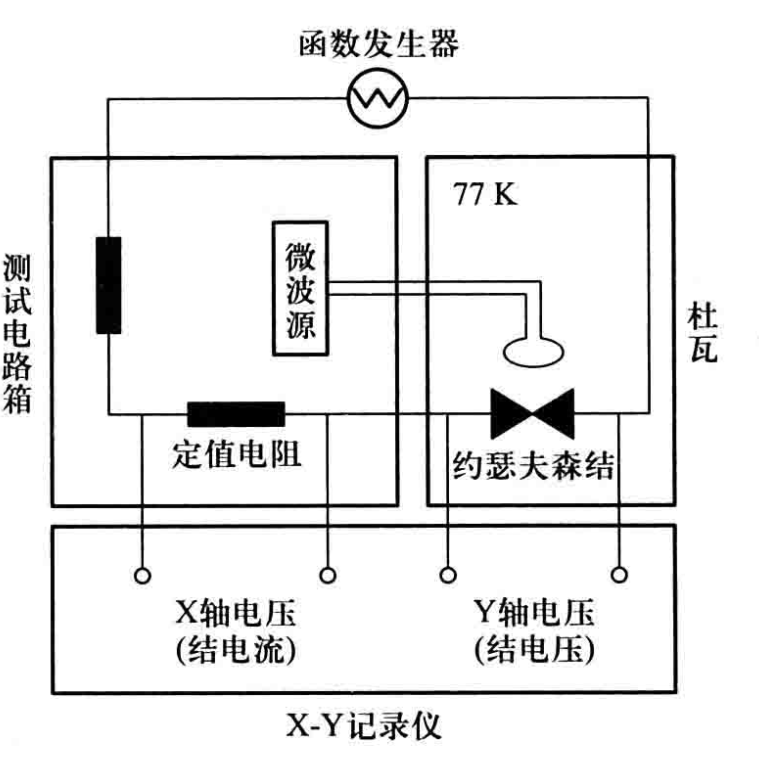
\includegraphics[width=0.85\linewidth]{fig/VIconnect.png}
  \caption{$V-I$曲线测量原理示意图
    % \note{推荐使用相对大小插入图片, 比如这里是 0.8 倍当前区域文字宽度 (\cs{linewidth}).
    %   推荐对实验装置图和数据图使用矢量图插入}
    }
  \label{fig:VIconnect}
  \end{figure}

  \par
  本实验的测量系统为$X-Y$记录仪. 需要注意的是, 实验中使用的该器材y轴旋钮和接线良好, 但x轴的细调旋钮损坏, 故实验中记录得到的x轴分度值并不准确, 需要通过其他手段进行校准, 具体操作见实验步骤说明.

% \note{这里使用了 \cs{autoref} 命令来自动给出带类型的交叉引用, 注意在命令前后适当使用空格以给出最好的显示效果.
%   小节, 表格, 公式等都可如此引用, 如: \autoref{sec:theory}, \autoref{ssec:table}, \autoref{sssec:table}, \autoref{eq:1}, \autoref{tab:table_eg}, \autoref{app:exercise}, \autopageref{tab:table_eg}.
%   交叉引用的标签尽量取得有意义.}

% 实验仪器和方法不是像普物实验报告那样将所有实验器材列出, 而是要用介绍功用的方式成段给出.
% 实验条件不仅是指直接影响实验结果的实验参量, 而且还包括影响实验质量和可靠性的因素, 如室温、空气湿度、基真空、原材料纯度等.

\subsection{实验步骤说明}
  由于本实验中双晶约瑟夫森结能承受的电流较小, 测量时为防止过大电流 (如静电) 损坏样品, 在非测量阶段需要把约瑟夫森效应观测仪 前面板上的“短路-测量”开关打到“短路”上, 准备就绪开始测量时, 再把开关打到“测量”状态.

  \subsection{测量双晶约瑟夫森结超导微桥的$R-T$曲线}
  \begin{enumerate}
    \item 初始化装置. 把待测样品放置于样品杆底部. 按照\autoref{fig:RTconnect}所示, 将$X-Y$记录仪与约瑟夫森效应观测仪后面板的相应接口连接. 将约瑟夫森观测仪的“短路-测量”开关打到“短路”位置, “$R-T$”和“$V-I$”开关打在“$R-T$”位置. 
    $X-Y$记录仪的x轴和y轴开关打到“Zero”位置. 把记录仪右下角的“Hold-Release”开关和“Up-Down”开关分别置于Release和Up状态, 将记录纸放到记录仪上, 使记录仪的两个红色指示灯分别在记录纸的同一条水平线上, 从而使得记录纸放正, 并把记录仪面板的“Hold-Release”开关置于Hold状态. 
    调整笔尖位置, 使得笔尖位于记录纸的左下角, 将记录仪的“Up-Down”开关置于“Down”状态, 打出坐标原点. 此后, 若需要移动记录纸, 只需将“Hold-Release”开关置于“Release”状态, 否则置于“Hold”状态; 若需要画图, 只需将“Up-Down”开关置于“Down”状态, 否则置于“Up”状态. 坐标原点最好取格点.

    \item 打开约瑟夫森效应观测仪的开关,  将$X-Y$记录仪的x轴和y轴开关打到“Measure”位置, $X-Y$记录仪的笔尖会移动至右上方. 调整X和Y方向的分度值, 使得笔尖位置不会超出仪器范围, 并尽可能在右上方. 使用万用表测量此时的铂电阻阻值, 从而得到此时的温度. 
    \item 将样品杆插入液氮罐中, 使样品浸没在液氮中, 此时样品温度下降. 等到记录仪笔尖不再移动时, 取下记录纸, 记录纸上会画出$V_J-V_T$曲线. 
    \item 结合x轴的坐标、y轴的坐标和分度值、恒流源输出电流、液氮的温度, 并利用77K\textasciitilde300K范围内铂电阻阻值几乎线性变化的物理规律即可得到超导转变点的温度. 
  \end{enumerate}

  \subsection{在液氮沸点下测量双晶约瑟夫森结的$V-I$曲线}
  \begin{enumerate}
    \item 将前面板的“短路”“测量”开关打到“短路”位置, 按照\autoref{fig:VIconnect}所示, 将$X-Y$记录仪与约瑟夫森效应观测仪后面板的相应接口连接. 把“$R-T$”和“$V-I$”开关打在“$V-I$”位置. 放好记录纸, 调整好笔尖位置、分度值 (本实验采用横坐标分度值为5mV/cm, 纵坐标分度值为10\mu V/cm). 
    \item 打开信号发生器, 使其输出频率为低频三角波 (本实验使用的是45mHz) , 逐渐增大输出电压幅值 (本实验使用的是3.272Vpp) , 同步调整分度值, 直到观测到约瑟夫森临界电流, 并画出优美的$V-I$曲线.
    \item 重新标定横坐标分度. 关闭约瑟夫森效应观测仪的开关, 移除其与$X-Y$记录仪的连接线, 将一电压源接在记录仪x轴输入端, 确定坐标原点, 调整电压源输出为1mV、2mV、3mv、4mv、5mv, 分别打点. 用尺子测量后点和点之间的距离并取平均值即可得到横坐标的分度值.
    \item 根据横坐标、横坐标分度和定值电阻阻值即可算出约瑟夫森临界电流.
    
  \end{enumerate}



  \subsection{在液氮沸点下施加微波辐照, 测量双晶约瑟夫森结的$V-I$曲线}
  \begin{enumerate}
    \item 在上一步实验的基础上, 连接微波辐照装置和样品杆并打开微波辐照.
    \item 调整微波辐照装置的频率和输出功率,$X-Y$记录仪的分度值, 观察$V-I$曲线的变化, 可以看到较为清晰的夏皮罗台阶.
    \item 根据纵坐标值及其分度、台阶个数等可以算出微波频率. 将其与仪器展示的频率对比, 验证约瑟夫森效应理论的正确性.
  \end{enumerate}


\section{结果及讨论}


  \subsection{双晶约瑟夫森结超导微桥的$R-T$曲线}
  实验得到的双晶约瑟夫森结超导微桥的$V_J-V_T$曲线如\autoref{fig:RT}所示. 其中, y轴分度值为0.1mV/cm, x轴显示的分度值为10mV/cm.
  \begin{figure}[htbp]
    \centering
    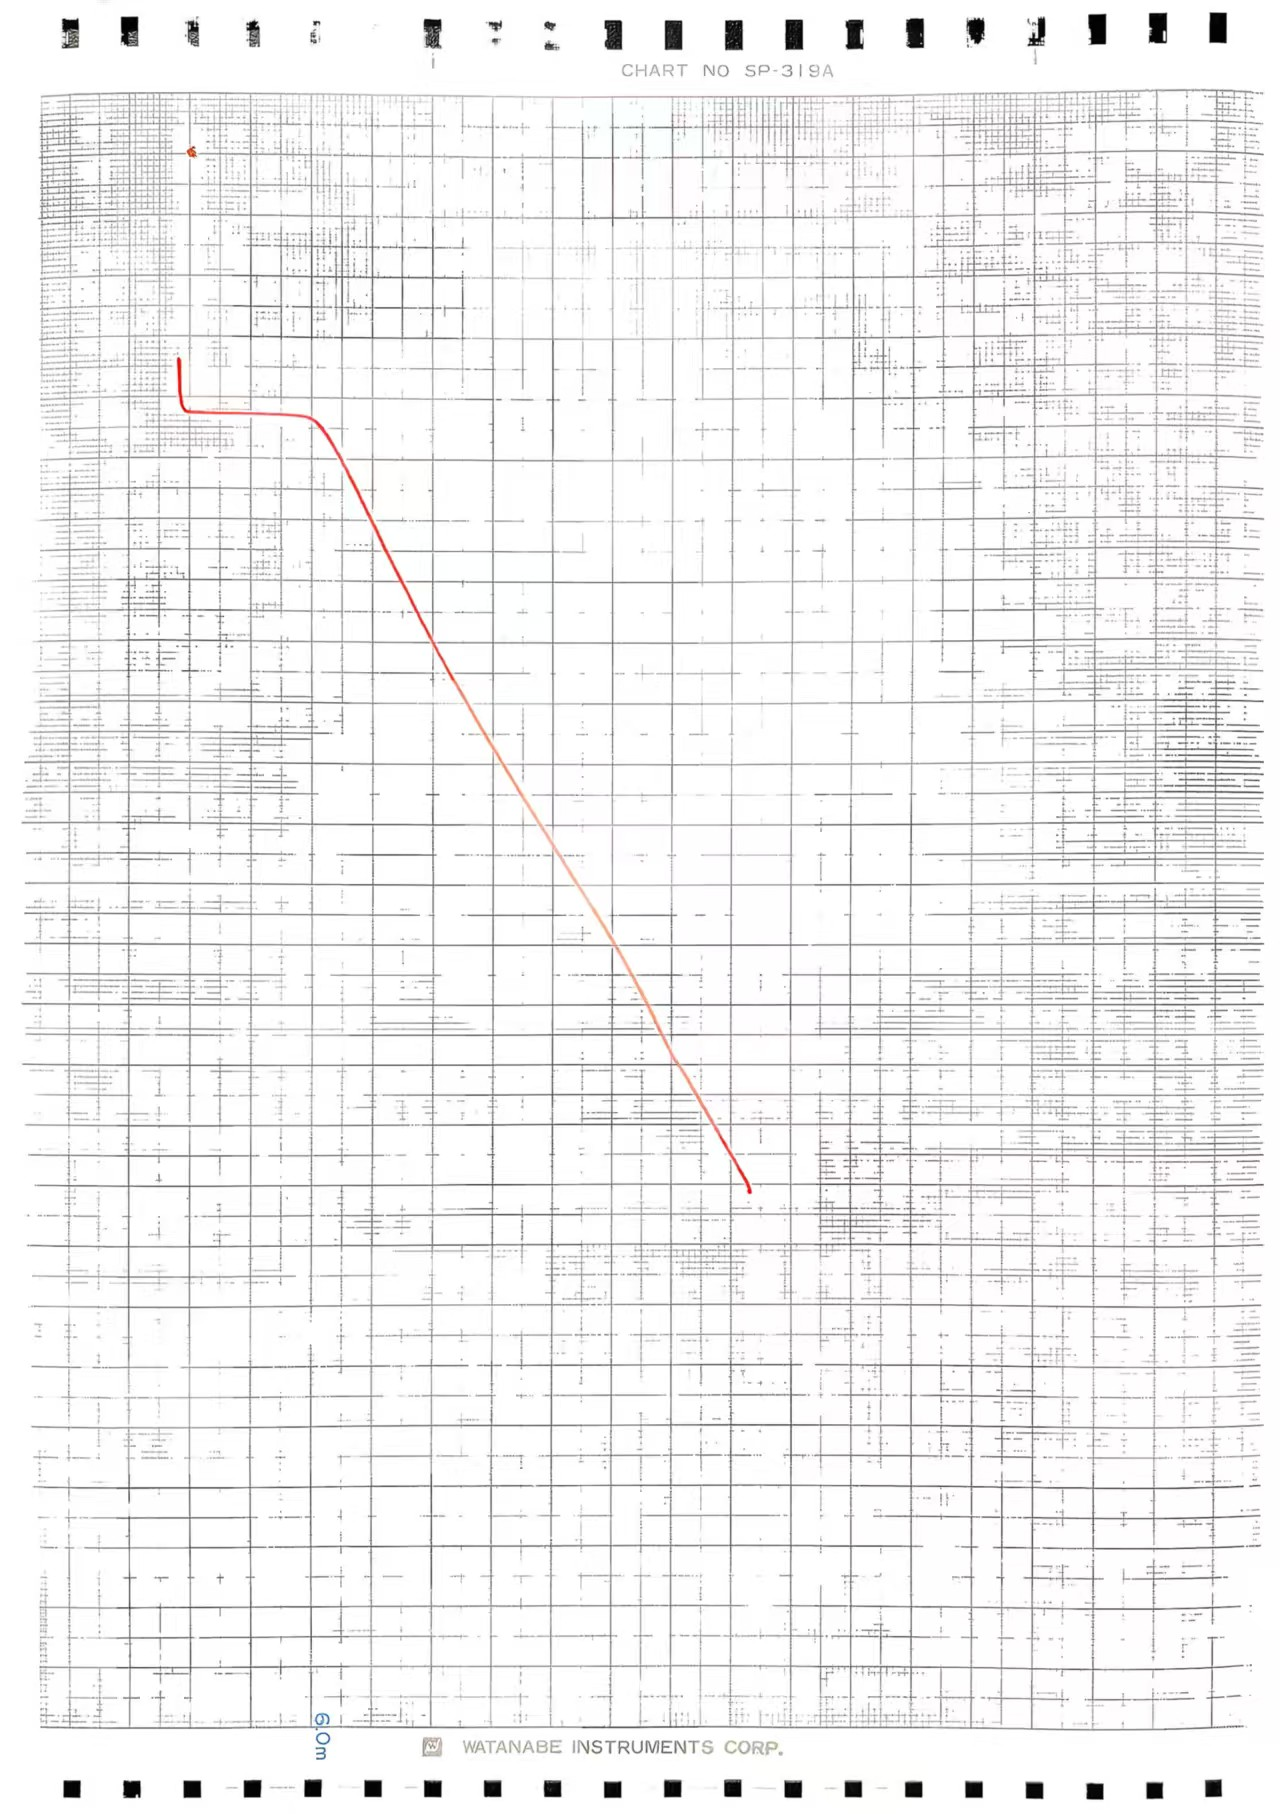
\includegraphics[width=0.85\linewidth]{fig/3.jpg}
    \caption{双晶约瑟夫森结超导微桥的$R-T$曲线}
    \label{fig:RT}
  \end{figure}

  测量得初始测量点的横坐标 (距离) 为17.16cm, 超导转变点的横坐标 (距离) 为4.22cm, 最终不变点的横坐标 (距离) 为3.35cm.
  室温下用万用表测量得到的铂电阻大小为109.6$\Omega$, 由此可查表并利用其线性计算得到此时的温度为297.715K.
  已知液氮温度为77K. 根据铂电阻阻值和温度的线性关系, 可以计算得到转折点的温度约为90.9K. 

  \par
  可以发现, 在液氮温度下, 约瑟夫森结两端的电压并不为0, 而是一恒定的负值. 这可能是由于实验装置所处的温度跨度较大而产生了温差势能, 或是诸如电压测量系统零点漂移等其他实验装置本身原因造成.


  \subsection{在液氮沸点下测量双晶约瑟夫森结的$V-I$曲线}
  实验得到的液氮沸点下双晶约瑟夫森结的$V-I$曲线如\autoref{fig:VI}所示. 其中, y轴分度值为10$\mu V/cm$, x轴显示的分度值为5mV/cm.
  采用外加电压源重新标定x轴分度, 得到x轴分度为7mV/cm.
   \begin{figure}[htbp]
    \centering
    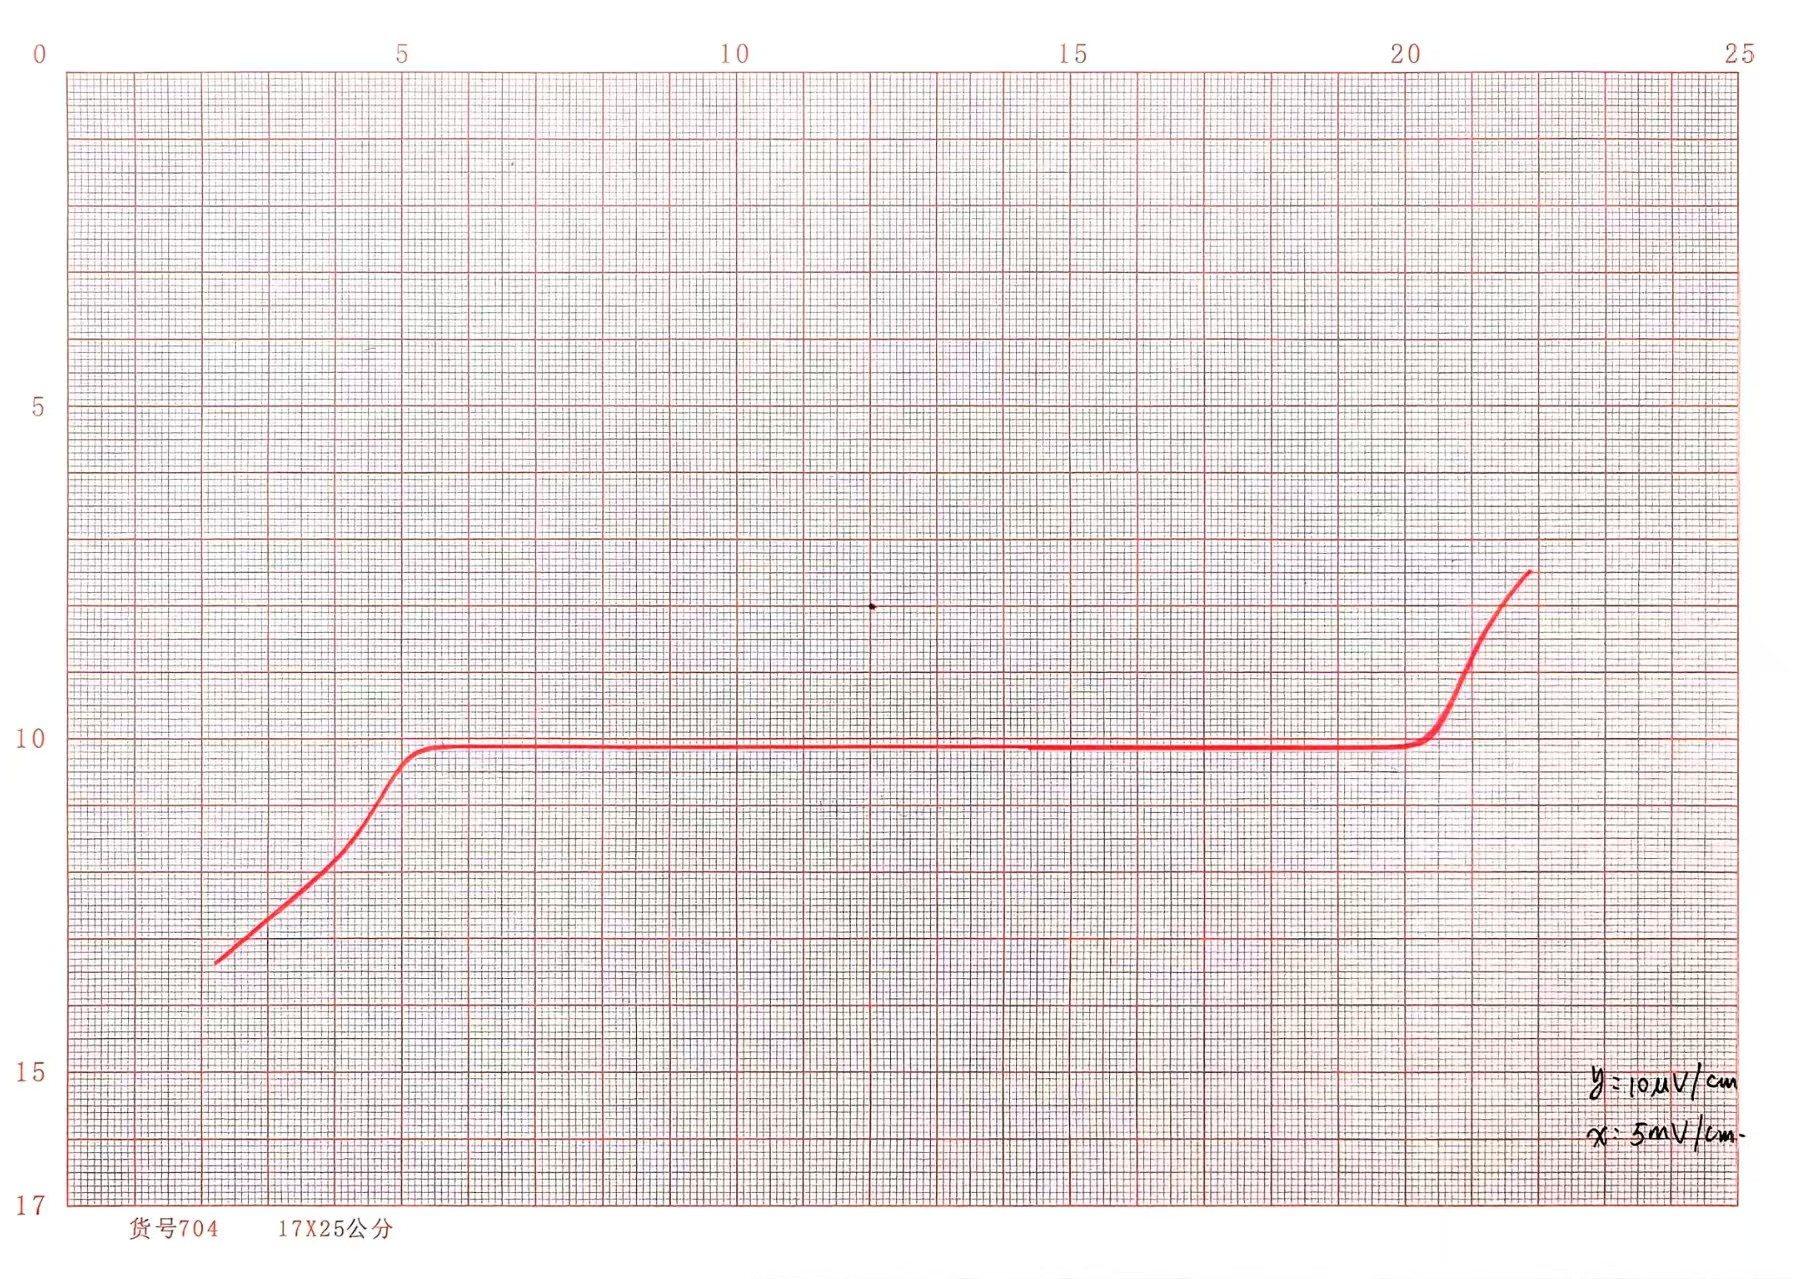
\includegraphics[width=0.85\linewidth]{fig/4.jpg}
    \caption{双晶约瑟夫森结无微波辐照下的$V-I$曲线}
    \label{fig:VI}
  \end{figure}

  测量得到两个转变点之间距离为14.31cm, 由此可以计算得到约瑟夫森结的临界电流为$I_c=\frac{14.31\times 7}{2\times 50}=1.0017mA$.

  \par
  当电流大小大于约瑟夫森临界电流时, 约瑟夫森结两端会出现电压差, 这是由于样品内电子发生隧穿导致的.

  \subsection{在液氮沸点下施加微波辐照, 测量双晶约瑟夫森结的$V-I$曲线}
  实验得到的液氮沸点下双晶约瑟夫森结在微波辐照下的$V-I$曲线如\autoref{fig:VI_mw}所示. 其中, y轴分度值为10$\mu V/cm$, x轴显示的分度值为5mV/cm.
  采用外加电压源重新标定x轴分度, 得到x轴分度为7mV/cm.
  从图中可以观察到较为明显的夏皮罗台阶.
  测量得到各个台阶的高度如表\autoref{tab:step}所示.
  \begin{figure}[htbp]
      \centering
      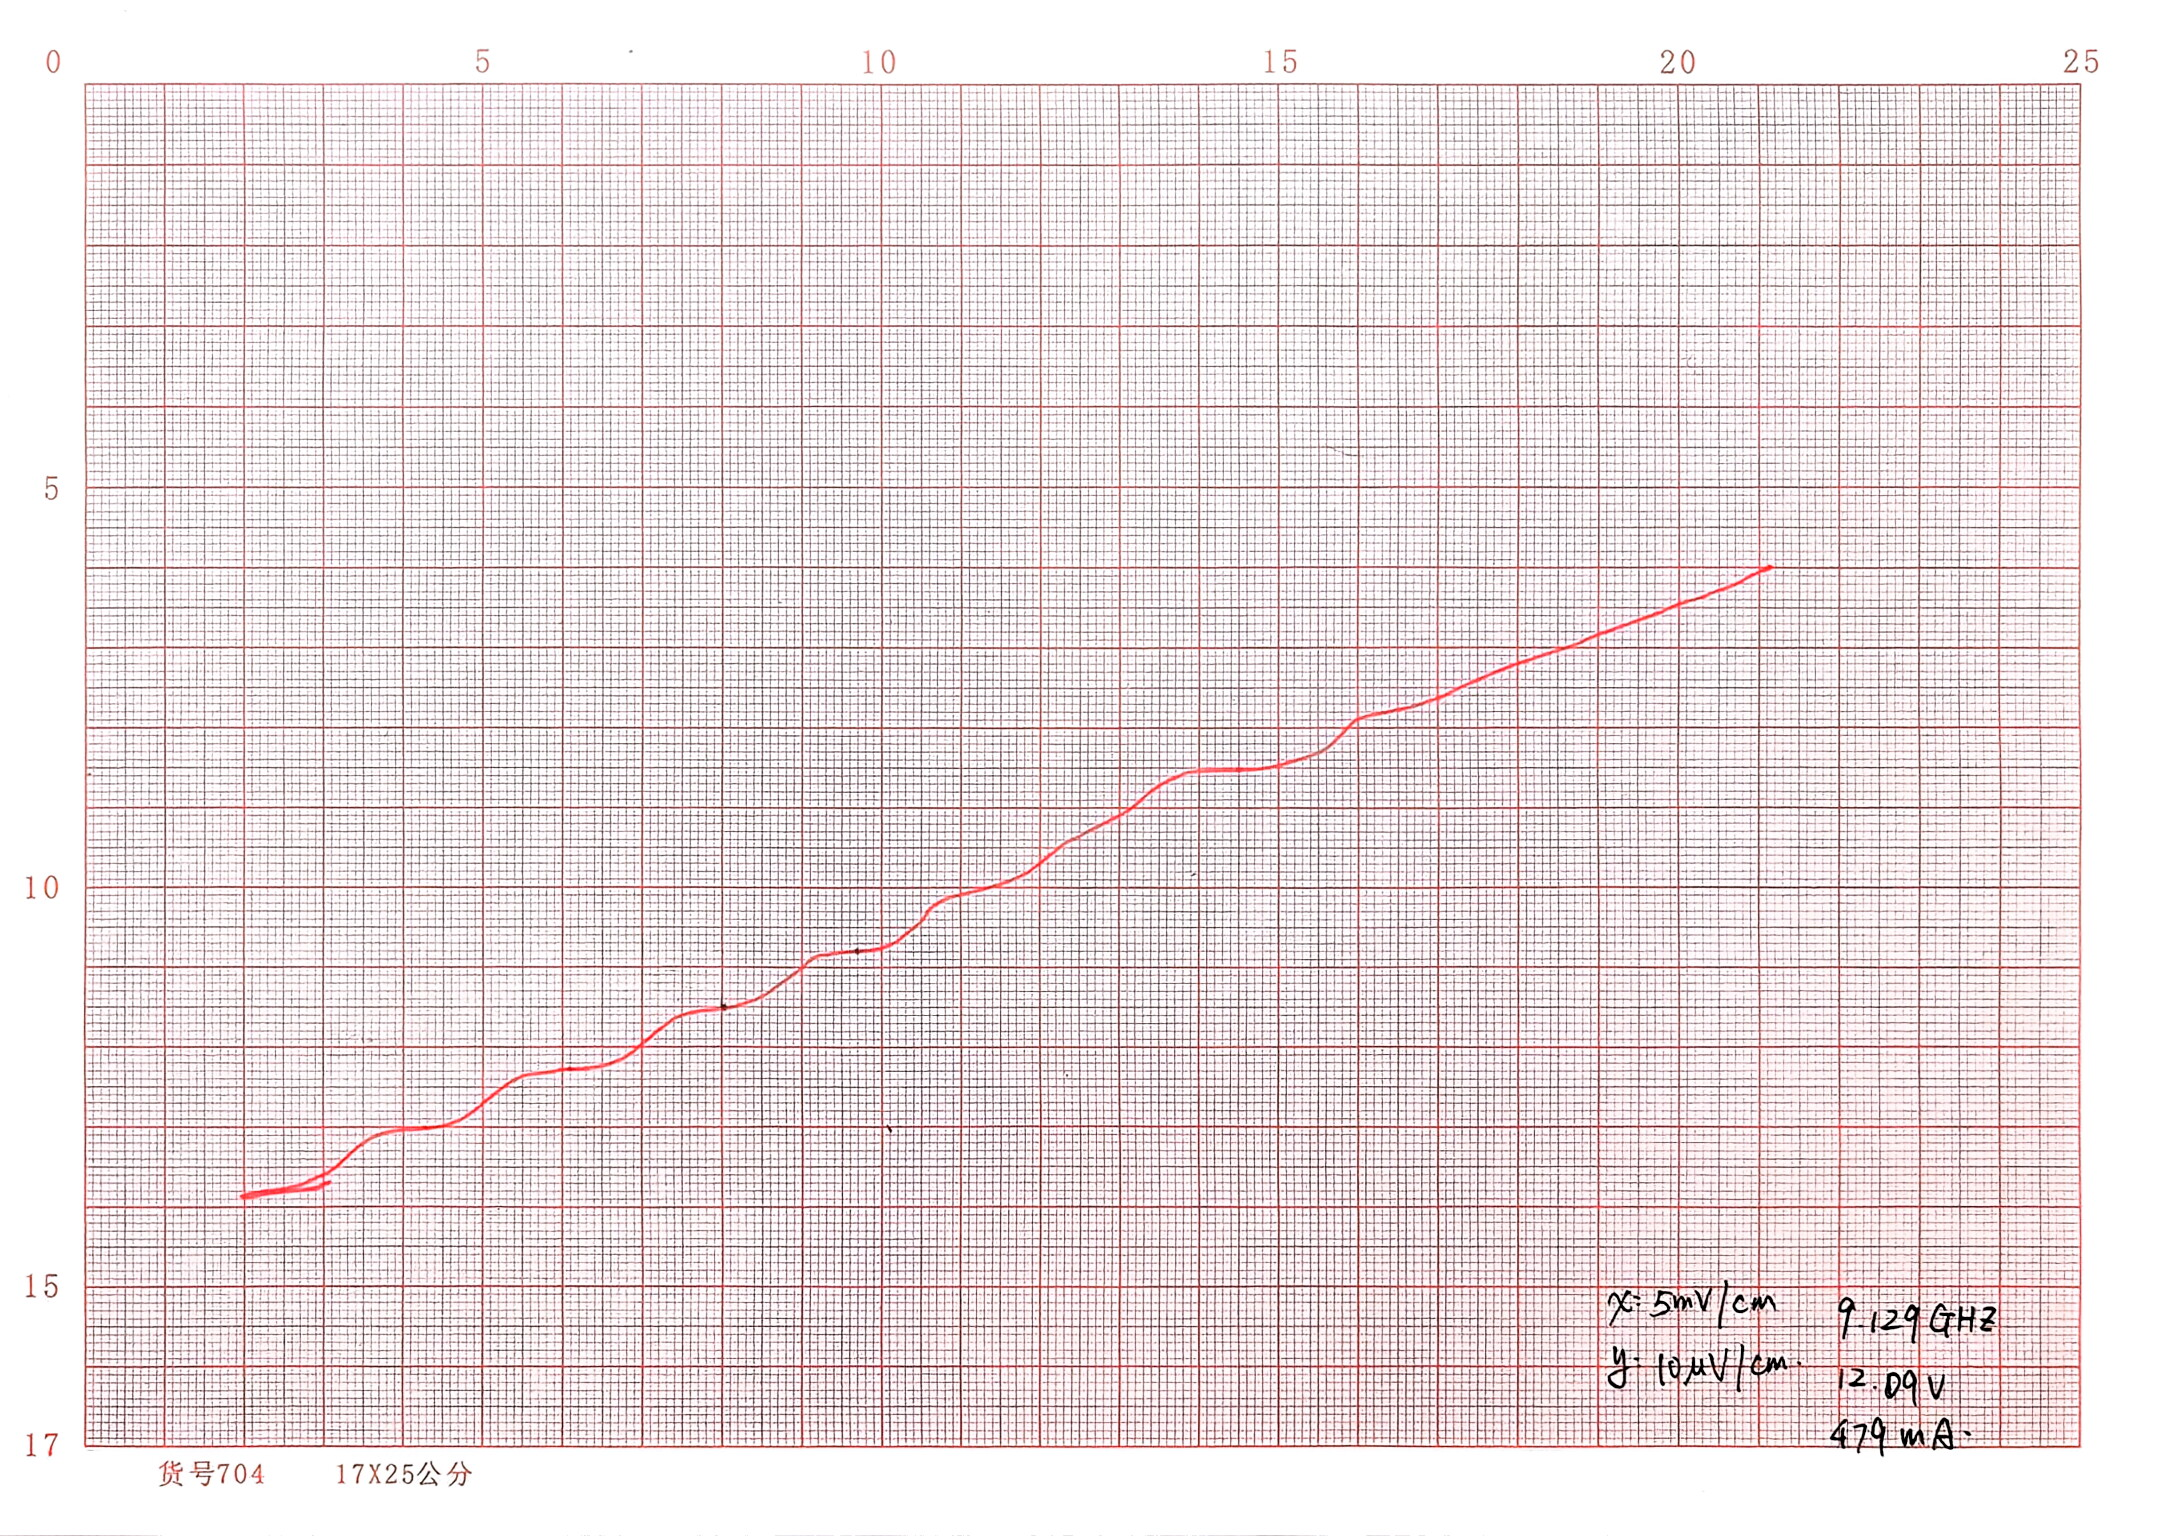
\includegraphics[width=0.85\linewidth]{fig/5.jpg}
      \caption{双晶约瑟夫森结无微波辐照下的$V-I$曲线}
      \label{fig:VI_mw}
    \end{figure}
  
  \begin{table}[htbp]
    \caption{夏皮罗台阶高度与序数的关系}
    \label{tab:step}
    \begin{ruledtabular}% ruledtabular 环境自动生成首尾双横线, 并调整宽度至占满全行
      \begin{tabular}{c|c|c|c|c|c|c|c}
        % d{a.b} 能使该列中的数据按小数点对齐, 前方留 a 个字符, 后方留 b 个字符
        % 已将 multicolumn 简写为 mc
        n  &  -3  &  -2  &  -1  &  0  &  1  &  2  &  3   \\
        \colrule% 中间横线
        y/cm     & -2.20 & 1.48 & 0.72 & 0 & 0.71 & 1.50 & 2.30 \\
        V/\mu V   & -22.0 & -14.8 & -7.2 & 0 & 7.1 & 15.0 & 23.0\\
      \end{tabular}
    \end{ruledtabular}
  \end{table}
  使用Origin对其作线性拟合, 得到如\autoref{fig:fit}直线, 拟合得到的斜率$k = 7.46017\mu V$. 
  \begin{figure}
      \centering
      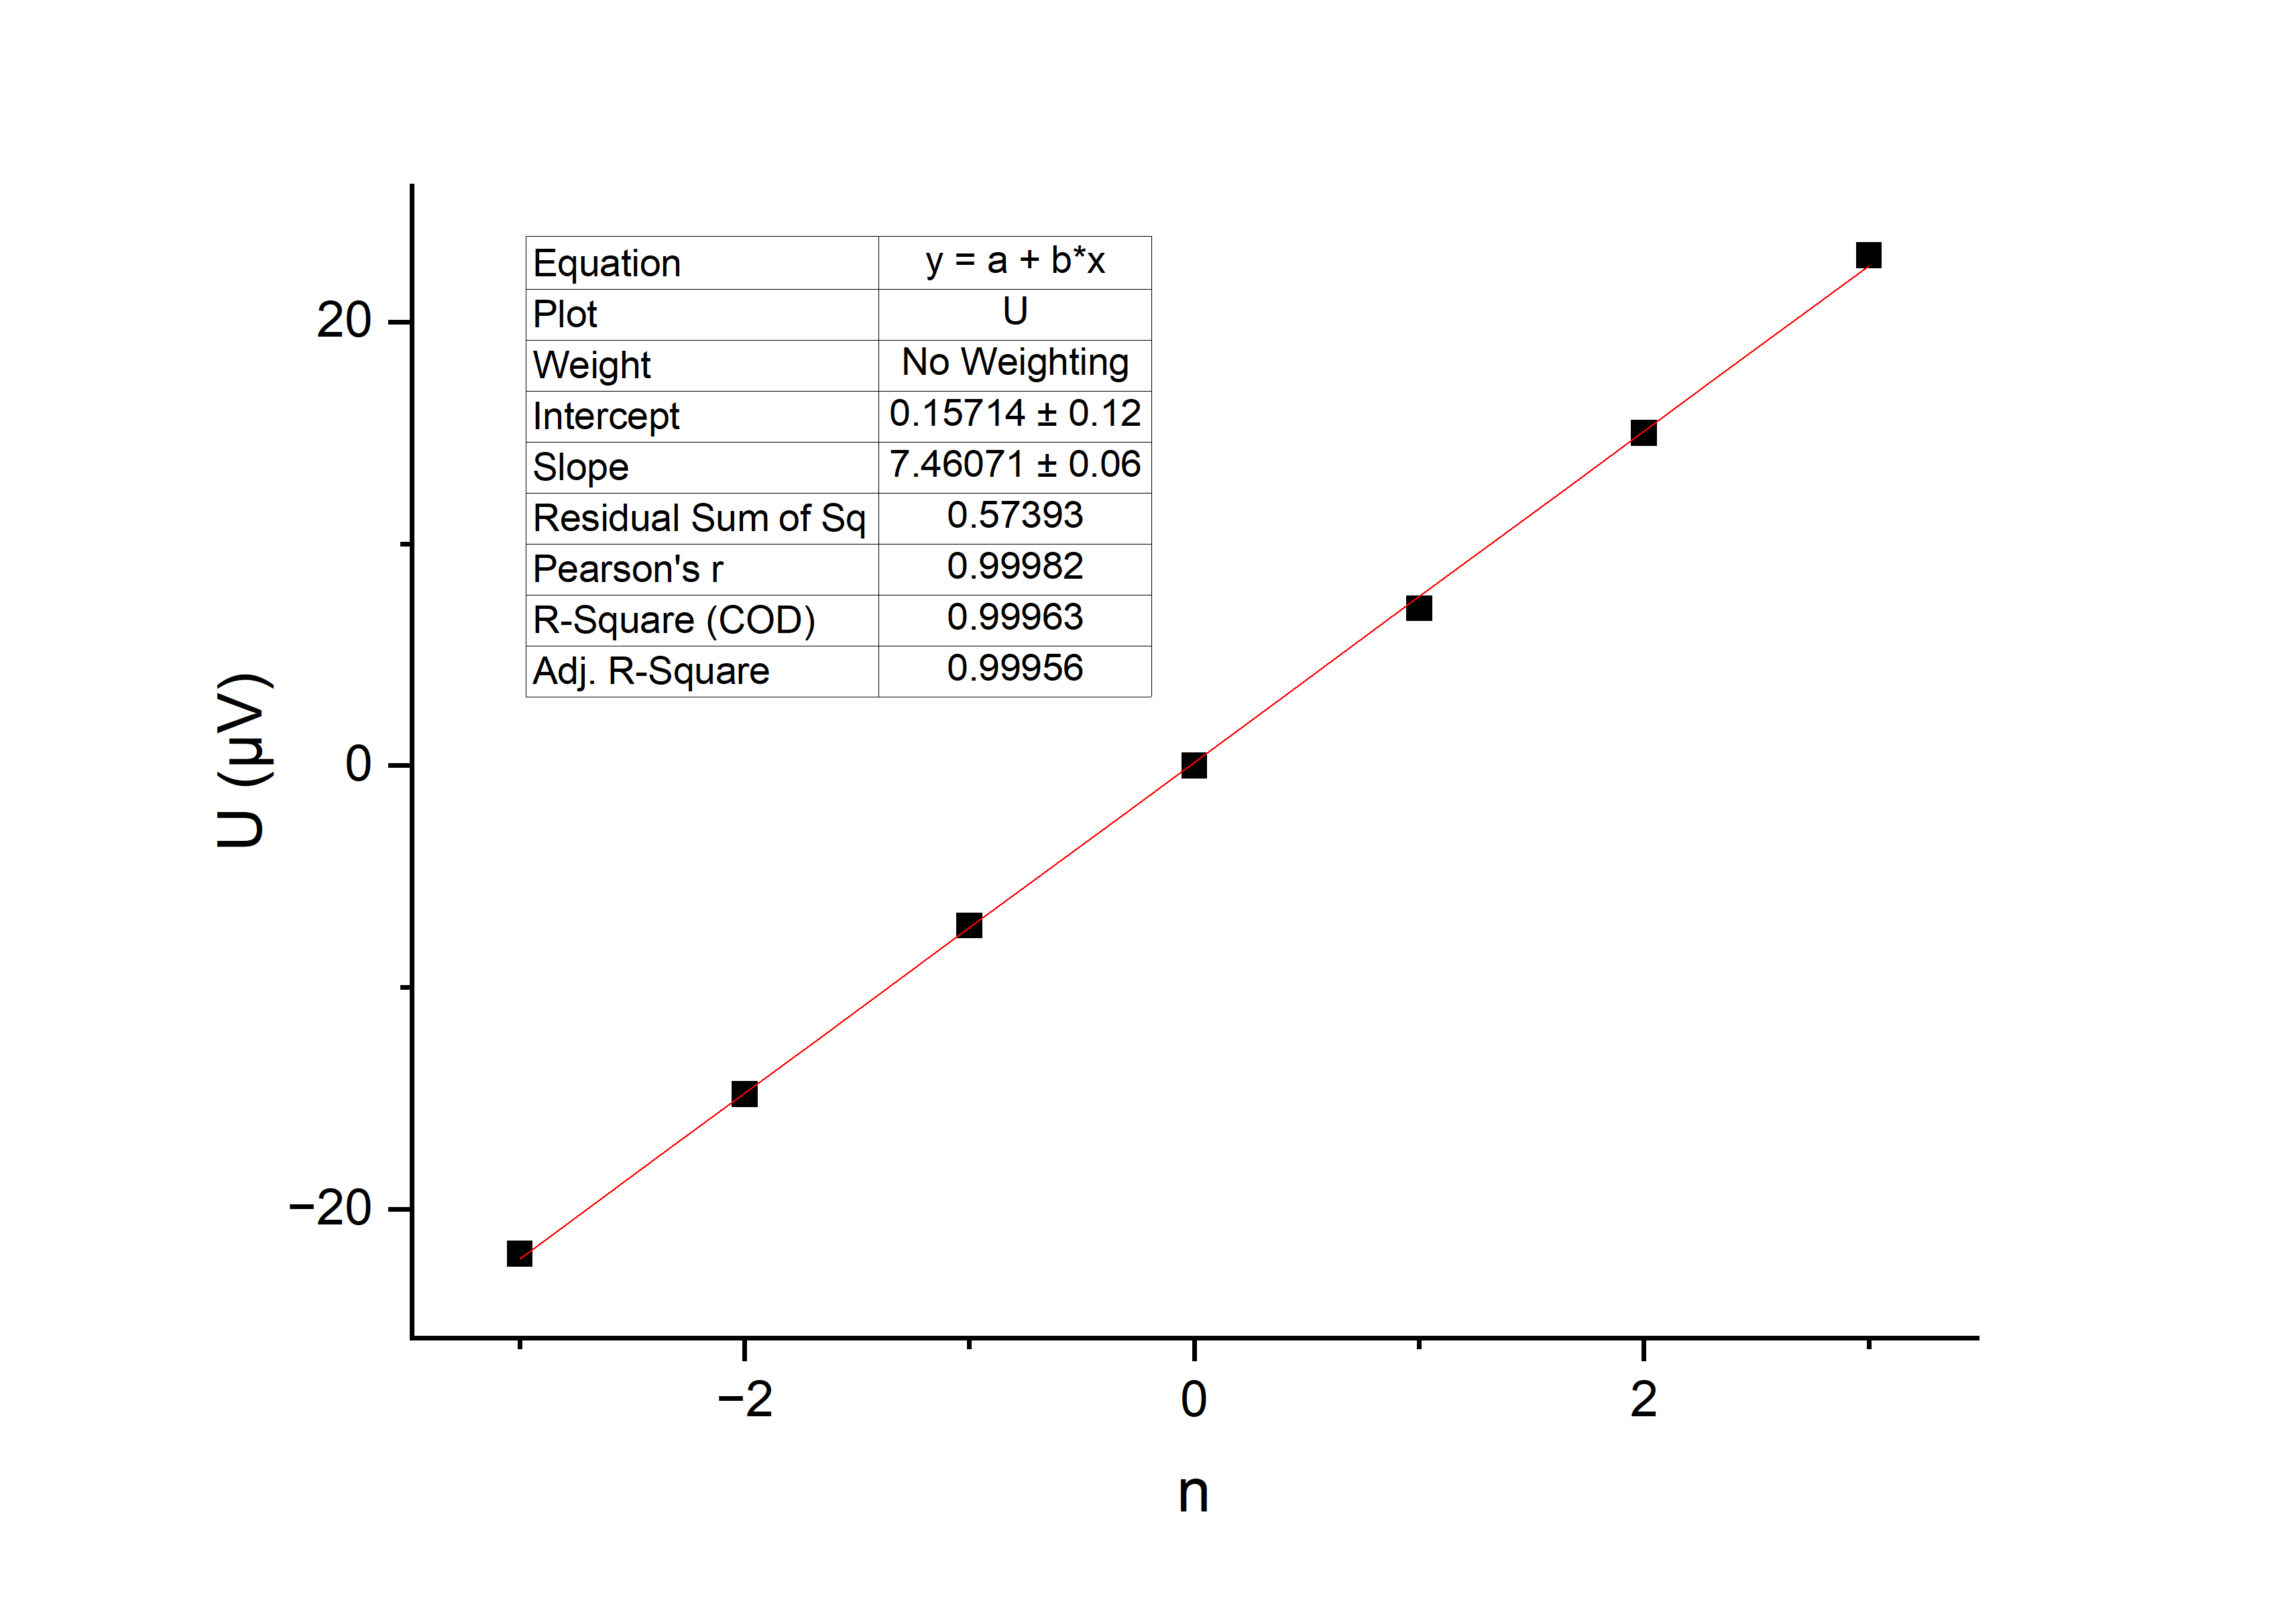
\includegraphics[width=0.85\linewidth]{fig/6.png}
      \caption{夏皮罗台阶高度与序数的关系拟合}
      \label{fig:fit}
  \end{figure}
  已知公式$ V = n\frac{h\nu}{2e}$, 由此得到$k= \frac{h\nu}{2e} $, 从而可以计算得到微波频率$\nu = \frac{2ek}{h} = 3.608GHz$.
  \par
  但是仪器实际显示的微波频率为9.129GHZ, 与理论计算的相差较大. 这可能是由以下几点原因造成的:
  \begin{itemize}
    \item 实验中记录的y轴分度值错误, 实际打到的分度值为$25\mu V/cm$而不是记录的$10\mu V/cm$. 推测该原因可能性较大, 因为实验中观察到y轴旋钮的指示线恰好位于$10\mu V/cm$和$25\mu V/cm$之间, 可能读数有偏差.
    \item 实验使用的$X-Y$记录仪除了x轴分度值损坏外, y轴分度值也可能存在误差.
    \item 在测量夏皮罗台阶的高度时, 误把二级台阶认为是一级台阶, 导致测量得到的台阶高度较小. 但是根据\autoref{fig:VI_mw}所示, 台阶较为明显, 误记的可能较小. 
  \end{itemize}
  如果根据第一点原因, 则重新计算得到的微波频率为9.02GHz, 与仪器显示的9.129GHz较为接近, 误差约为1.2\%. 
  \par
  由此可以验证约瑟夫森效应理论的正确性.
  \par
  如果使用不含双晶结的超导微桥样品进行试验, 理论上记录得到的无微波辐照和有微波辐照的$V-I$曲线都是一条直线, 即不存在约瑟夫森效应.
  这是因为对于$YBa_2Cu_3O_{7-x}$, 其相干长度极小, 无双晶结的样品很难在样品间形成弱耦合, 导致无法产生约瑟夫森效应. 
  而双晶衬底的约瑟夫森结是由两块平行于衬底表面晶向不同的的$YBa_2Cu_3O_{7-x}$粘合形成, 可以使得两块超导体间形成弱连接, 产生约瑟夫森效应.



% 此部分是实验报告的主体, 应占报告篇幅的一半以上.
% \note{依自己意愿, 结果与分析部分可以分多个小节, 甚至可以将实验结果和对结果的分析讨论拆分为两节.}

% 实验结果应尽量以图表的形式给出. 每一个图表都应该是完整的, 即阅读图表时可以不必依赖正文.
% 以图表为中心叙述实验结果和讨论.

% \subsection{表格}\label{ssec:table}
% \subsubsection{表格}\label{sssec:table}


% 表是被一系列横线隔开的有序排列的数据, 报告格式要求最上和最下两条横线为双横线.
% \note{此双横线格式可以通过 \env{ruledtabular} 环境和 \cs{colrule} 命令实现.}
% 例表为\autoref{tab:table_eg}.

% \begin{table}
%   \caption{表格示例%
%     \footnote{表格标题要简明扼要; 注意使用 \pkg[revtex]{revtex4-2} 提供的 \env{ruledtabular} 环境生成首尾双横线的表格.
%       表格中的脚注会自动加在表尾.
%       为方便, 提供了 \cs{mc} 作为 \cs{multicolumn} 的简写.
%       \href{https://www.tablesgenerator.com}{Tables Generator 网站}可以方便地生成 \LaTeX 表格.}}
%   \label{tab:table_eg}
%   \begin{ruledtabular}% ruledtabular 环境自动生成首尾双横线, 并调整宽度至占满全行
%     \begin{tabular}{cd{4.2}lr}
%       % d{a.b} 能使该列中的数据按小数点对齐, 前方留 a 个字符, 后方留 b 个字符
%       % 已将 multicolumn 简写为 mc
%       居中    & \mc{1}{c}{数值 %
%         \footnote{``数值'' 列使用了 \code{d} 列格式来按小数点位置对齐.
%         记得将 \code{d} 列的列标题单独设为居中.
%         \pkg{siunitx} 提供了更为复杂的小数点对齐功能, 请参考其文档.}
%       }     & 靠左           & 靠右 \\
%       \colrule% 中间横线
%       a     & 0.12         & a     & a \\
%       bbb   & -100         & bbb   & bbb \\
%       ccccc & 50.8         & ccccc & ccccc
%     \end{tabular}
%   \end{ruledtabular}
% \end{table}

% 从\autoref{tab:table_eg} 可以看出, 对表中各项的注释应作为表的一部分放在表后, 而不是页脚或文尾.
% \note{在表格中使用 \cs{footnote} 命令时 \LaTeX 会自动将注释放在表尾.
%   但正文中的注释按照 AIP 的要求 (以及 \pkg[revtex]{revtex4-2} 的实现) 是会和各引用项共同编号并作为参考文献列表的一部分的.
%   因此, 只要你在正文使用了 \cs{footnote}, 即使你没有引用任何文献 (这一般不太可能), 也需要用 B\textsc{ib}\TeX 处理.
%   这里是一个尾注的例子 \footnote{这里是一个尾注的例子}.}

% 当原始数据和处理过的数据常需要出现在同一表中时, 用软件来处理会非常方便.
% 但出现在实验报告中的表应具有上面给出的例子的格式.

% \subsection{数据图}

% \textbf{每个图应尽量让读者不看正文就能基本理解图的含意.}
% 应包含: 图名、轴名、轴、刻度、标尺、数据点、曲线、图例、标注和图注等部分.
% 最常用的作图软件有 Origin 或 MATLAB.
% 学习使用基本的数据处理和作图工具软件也是课程的基本内容.
% 课程也鼓励大家使用 Python 语言编程作图.
% 逐点测量得到的函数关系要同时用表格和图给出.
% \note{数据点过多可以将数据放到附录.
%   这里 ``逐点测量得到的函数关系'' 还是要自己把握一下, 像那种几千个数据点的能谱当然就没必要放原始数据表了.}
% \textbf{需要作比较的多条曲线要画在同一图上.}
% 为避免读者在图表和正文间反复跳跃阅读, 正文叙述应紧邻图表, 正文中也要对图表作必要的说明.

% \begin{figure}
%   \centering
%   \includegraphics[width=0.8\textwidth]{fig/figsample.pdf}
%   \caption{这是数据图的例子.
%     \note{在图的 \cs{caption} 中应简要说明图中表达的内容, 并对各种符号、线型、颜色的意义做出说明.
%       如果有多格数据图, 应清晰地分别做出解释说明.
%       图中的关键性文字 (比如轴名和图例) 的大小最好能和说明文字中的文字大小相当.
%       关于坐标轴名和单位的标法, 可以参看\href{https://journals.aps.org/authors/axis-labels-and-scales-on-graphs-h18}{美国物理学会的说明}.
%       本图是用脚本 \file{figgen.py} 生成的}}
%   \label{fig:data}
% \end{figure}

% \autoref{fig:data} 是一张例图.

% \subsection{对分析的要求}

% 对于预料之外的实验结果, 必须首先小心证明其可靠性.
% 读者只有在相信你的实验结果时才愿意花时间看你的分析.

% \textbf{必须用文字归纳整理出正式的实验结果或结论.}
% 可信的实验结果是课程报告最重要的内容.
% 作为一个实验物理工作者, 分析解释出错并不丢脸, 实验结果不被采信则是致命的.
% 教学实验的结论往往是预先知道的.
% 所以, 教师更关心的是你的说理过程.
% 一般说来, 单由课内实验的结果不足以能得到明确的结论.
% 此时, 你可以引用他人的研究结果来帮助帮助自己的论证, 但必须注明出处.
% 确实不能得到明确结论时, 可以给出几种可能结论并指出可以再做哪些实验来帮助作进一步的判断.
% 总之, 分析讨论部分要做到: 论据要valid, 论证要reasonable, 结论要convincing.

\section{结论}
本实验使用双晶约瑟夫森结样品, 测量了其电阻与温度的关系曲线, 得到了其超导转变温度. 然后, 在液氮温度下, 测量得到了其在无微波辐照下的$V-I$曲线,
并得到了约瑟夫森临界电流. 最后, 给样品加以微波辐照, 测量得到样品的$V-I$曲线, 观察得到了较为明显的夏皮罗台阶, 并由此计算得到了微波频率, 验证了约瑟夫森效应理论的正确性.

% 首先要给出实验结果, 然后再给出由实验结果分析得到的结果和结论.
% 此部分给出的内容要比摘要中的全面, 用词要更准确.

\begin{acknowledgments}
  感谢王越老师的耐心指导和帮助.
  \par
  感谢搭档王天天同学的协助.
  % 感谢对实验和报告有具体重要帮助的, 又没被列为作者的人.
  % \note{撰写致谢时请使用 \env{acknowledgments} 环境.}
\end{acknowledgments}

% bibliography 的参数是你的 *.bib 文件去掉后缀名后的部分
\bibliography{bibli}

\clearpage % 附录前另起一页
\appendix % 附录开始
\section{思考题}\label{app:exercise}
\subsection{在进行$R-T$曲线测量时如何选定坐标记录原点和$R-T$记录仪的分度值以得到合适的测量曲线?}
坐标原点尽可能选在左下角的格点上. 在样品温度在室温时, 将$X-Y$记录仪的x轴和y轴分别调到Measure档, 调整x轴和y轴的分度值, 使得笔的位置尽可能在纸的右上角, 但是又不超出仪器记录范围.
这样做的目的是让记录得到的图像尽可能铺满全纸, 原点在格点方便测量距离.
\subsection{通过测量$V-I$曲线来考察直流约瑟夫森效应时,$X-Y$记录仪轴 (结电压) 的分度值在开始时应该选定在什么挡位?是应该大还是应该小? }
y轴分度值取值应该尽可能小, x轴分度值应该要使得横向的图像不能超出纸的范围. 
\subsection{随着微波输出功率的变化,双晶约瑟夫森结的伏安特性 ($V-I$) 曲线有什么变化?产生的原因是什么?}
当$ V = n\frac{h\nu}{2e}$时, $\bar{j(t)} = (-1)^nj_cJ_n(\frac{2eu}{h\nu})\sin{\phi_0}\propto J_n(\frac{2eu}{h\nu})$.
\par
根据\autoref{fig:Bessel}所示, 随着u的增大, $J_0$的大小先减小后增大, $J_n (n\ge 1)$的大小先增大后减小. 即当功率逐渐增大时, 0级台阶的长度先减小后增大, 其余级别台阶的长度先增大后减小.
实验中也确实观察到了类似现象.
\begin{figure}
    \centering
    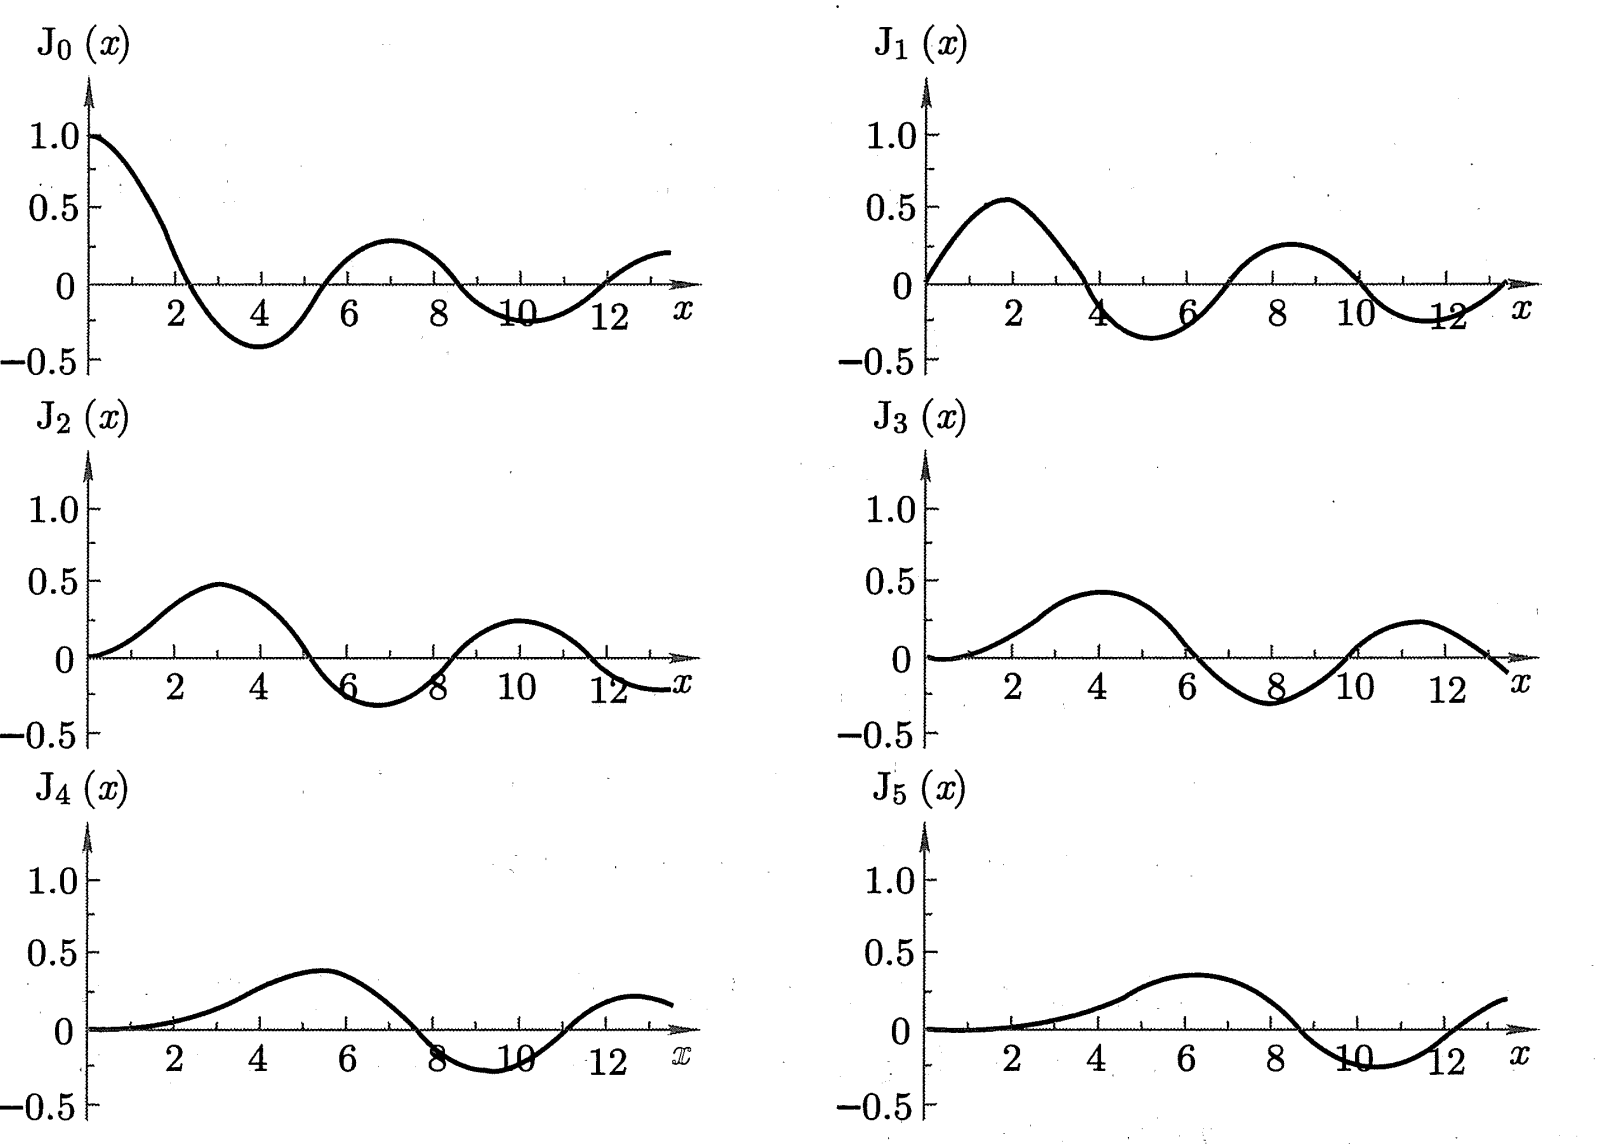
\includegraphics[width=0.85\linewidth]{fig/7.png}
    \caption{自变量为实数时的Bessel函数 (摘自\cite{shulifangfa})}
    \label{fig:Bessel}
\end{figure}

\subsection{双晶结超导微桥与不含有双晶结的超导微桥的测量结果有什么差异? 这些差异为什么可从一个侧面证实约瑟夫森效应的观测? }
双晶结超导微桥在没有微波辐照时, 当电流超过约瑟夫森临界电流时, 电压不为0; 在有微波辐照时, 会出现夏皮罗台阶. 而不含有双晶结的超导微桥的电压在测量范围内始终是0. 
得到的约瑟夫森临界电流大小远小于超导临界电流, 可以从侧面证实
约瑟夫森效应观测.
夏皮罗台阶的观测也可以反映交流约瑟夫森效应.


\subsection{为什么说超导是宏观量子现象?通过此实验, 谈谈你对这个问题的理解. }
约瑟夫森效应原理是库珀对的隧穿效应, 这属于量子现象. 但是它可以通过宏观的电流、电压观测得到. 所以是宏观量子现象.

\subsection{约瑟夫森效应有哪些应用 (你了解或设想的), 这些应用的基本原理是什么? }
约瑟夫森效应有诸多应用, 比如绝对电压基准、超导量子比特等. 其中, 绝对电压基准原理是微波感应台阶电压和频率的一一对应关系, 而频率可以被原子钟等精确测量, 因此可以得到基准电压.
超导量子比特的基本原理是约瑟夫森结可等效为一个 “超导量子干涉器件” (SQUID) , 其核心是 “电荷 - 磁通” 的量子化特性. 结的超导电流状态 (如电流方向、大小) 对应量子态的不同能级,可通过外部磁场或电压调控这些量子态,实现量子比特的 “0” 和 “1” 状态。


% \section{近代物理实验报告写作要求}

% 物理实验的结果最终需要以论文或报告的形式向同行或公众报道.
% 外界也主要基于这些论文或报告来评价一个实验物理工作者.
% 所以, 课程实验报告的撰写是北大 ``近代物理实验'' 课的一个重要内容和主要的评分依据.

% 北大近代物理实验课要求按研究论文的形式来撰写课程实验报告.
% 和任何期刊一样, 近代物理实验课对学生提交的课程实验报告也有内容和格式上的要求.
% 学生应依照课程提供的课程实验报告模板来撰写自己的实验报告.

% 课程提供的课程实验报告模板综合了 American Institute of Physics (AIP) 期刊和中国《物理学报》对稿件格式的要求.

% 本实验报告模板各部分的文字给出了相应节写作时应注意的问题.

% \subsection*{报告写作的一般事项}

% \begin{enumerate}
%   \item 课程实验报告应假定读者既不是已知全部实验细节的指导教师, 也不是缺少专业知识的公众, 而是同领域的实验研究者, 或审稿人.
%         不能要求读者要在读过课程讲义后才能读懂课程实验报告.
%   \item 文本和物理量单位用正体, 物理变量符号用斜体, 矢量矩阵符号用黑斜体.
%         \note{(\pkg{physics} 宏包提供了大量的方便的物理中常用符号的排版工具, 请参考其文档使用)}
%   \item 使用国际标准的缩略词, 符号和法定计量单位时应全文一致, 正文中的缩略
%         词在\textbf{首次出现时写出全称}, 后附缩略词, 并用括号括起; 之后直接用缩略词, 不
%         再写全称, 如 American Institute of Physics (AIP).
%   \item 全文标点符号除 ``顿号'' 外, 其他用英文半角标点符号.
%         \note{(推荐的格式中, 英文单词和数字应与汉字之间插入一个空格;
%           半角标点符号应如英文一般, 在逗号, 句号, 分号等后方插入一个空格;
%           在引号, 括号外侧各插入一个空格;
%           连续出现的标点符号之间的多余空格则应删除.
%           但是, \pkg{xeCJK} 宏包基本上自动为你在最终的 PDF 文稿中完成了这些事情.
%           此外, 如果你觉得半角符号配中文太丑, 请参见 \file{README.md} 中介绍的标点选项)}
%   \item 公式、图和表要分别用阿拉伯数字编列序号. \note{(这点 \LaTeX 可以为你代劳)}
%         公式和图表要达到可发表的质量.
%   \item 凡不是自己独立思考得到的内容都应该引参考文献.
%         不能大段引用同一参考文献.
%         对复杂问题, 应该优先考虑引用参考文献得到结果.
%         对简单一些的问题才鼓励独立思考.
%         只能引用正式出版物, 不能引用他人实验报告.
%   \item 模板中的未尽事项可以参考 AIP Style Manual 4th-edition (可从课程网站下载).
%         \note{(也可参考 \pkg[revtex]{revtex4-2} 的文档)}
%   \item 较长的推导和说明可以作为附件提交, 不占用报告篇幅.
%   \item 思考题不是报告的组成部分.
%         应另起一页附在报告的最后. \note{(比如作为附录)}
% \end{enumerate}

% \section{对 \LaTeX{} 中标点输入的额外说明}
% \LaTeX 中对 dash 有所区分,
% \begin{center}
%   \begin{tabular}{c@{\quad}c@{\ $\rightarrow$\ }c}
%     连字符 hyphen    & \verb|co-operate|     & co-operate \\
%     连接号 en-dash   & \verb|14--19|         & 14--19 \\
%     英文破折号 em-dash & \verb|Yes---or no?| & Yes---or no? \\
%     减号            & \verb|$-1$|           & $-1$ \\
%   \end{tabular}
% \end{center}
% 中文破折号 (——) 就按一般习惯的用输入法输入即可.
% \note{其实中文破折号就是两个连着的 em-dash, 但两种输入方式使他们输出字体不同.}

% \LaTeX 中半角引号使用如下映射进行输入.
% 左引号的符号为 \textsf{Esc} 键下方的锐音符.
% \begin{center}
%   \begin{tabular}{c@{\quad}c@{\ $\rightarrow$\ }c@{\quad}c@{\ $\rightarrow$\ }c}
%     单引号      & \verb|`|     & `     & \verb|'|     & ' \\
%     双引号      & \verb|``|    & ``    & \verb|''|    & '' \\
%     美式连续嵌套引号 & \verb|```|   & ```   & \verb|'{}''| & '{}'' \\
%     英式连续嵌套引号 & \verb|`{}``| & `{}`` & \verb|'''|   & ''' \\
%   \end{tabular}
% \end{center}
% 注意其中 \code{\{\}} 起到的分组作用.

% 此外, 如果想使用全角符号同时想使用实心点格式的句号, 可以使用 \code{quanjiao} 选项.
% 源文档中的 ``。'' 会被自动替换成 ``.''.
% 这时, 也就可以风格统一地直接使用中文输入法给出的引号 ``“”‘’'' 而不用管前面提到的映射了.
% 具体请参见 \file{README.md} 中介绍的标点选项.

% \note{其实“和``以及”和''分别是同一个 Unicode 字符, 只是被分配了不同的字体.}

% \section{DIY 字体效果测试}

% \newcommand{\testword}{报告}
% \newcommand{\andbold}{\testword{}\textbf{\testword{}}}
% \newcommand{\testline}{\testword{}\emph{\andbold{}}\andbold{}}

% 下面分别展示衬线, 无衬线和等宽中文字体效果, 便于检查基线高度等问题.
% \begin{center}
%   \textrm{\testline}\\
%   \textsf{\testline}\\
%   \texttt{\testline}
% \end{center}

\end{document}
